\documentclass[border=10pt]{standalone}
% Shared visual language for CAML diagrams (pdflatex + Fira Sans/Mono).
% Native SVG output: build with latex (DVI) + dvisvgm, see build.sh. The
% PDF route (pdflatex + dvisvgm --pdf) turns every transparency into solid
% black/white blocks.
\def\pgfsysdriver{pgfsys-dvisvgm.def}
\usepackage[T1]{fontenc}
\usepackage[sfdefault]{FiraSans}
\usepackage[scale=0.92]{FiraMono}
\usepackage{amssymb}
\usepackage{tikz}
\usetikzlibrary{arrows.meta, positioning, shadows, fit, backgrounds, calc}

% --- palette ------------------------------------------------------------
\definecolor{ink}{HTML}{16202C}
\definecolor{muted}{HTML}{5B6B7F}
\definecolor{edge}{HTML}{47576B}
\definecolor{card}{HTML}{F7F9FC}
\definecolor{page}{HTML}{FFFFFF}

\definecolor{indigo}{HTML}{4B54C6}   \definecolor{indigobg}{HTML}{EDEEFC}
\definecolor{amber}{HTML}{C9740A}    \definecolor{amberbg}{HTML}{FCF0DE}
\definecolor{green}{HTML}{0E9E6B}    \definecolor{greenbg}{HTML}{E4F6EE}
\definecolor{purple}{HTML}{7A3CE0}   \definecolor{purplebg}{HTML}{F1E9FD}
\definecolor{rose}{HTML}{D23F72}     \definecolor{rosebg}{HTML}{FBE7EE}
\definecolor{slate}{HTML}{47576B}    \definecolor{slatebg}{HTML}{EDF1F6}

% --- node + arrow styles ------------------------------------------------
% A flat offset drop shadow: shadows.blur's faded shadows render as solid
% black boxes under the dvisvgm driver.
\tikzset{soft shadow/.style={drop shadow={shadow xshift=0pt, shadow yshift=-1.8pt,
                                          opacity=0.12, fill=ink}}}
\tikzset{
  base/.style={
    rounded corners=5pt, draw, line width=1pt, inner sep=8pt,
    font=\small, text=ink, align=center,
    soft shadow},
  card/.style   ={base, fill=card,     draw=muted!70},
  indigo/.style ={base, fill=indigobg, draw=indigo, text=ink},
  amber/.style  ={base, fill=amberbg,  draw=amber,  text=ink},
  green/.style  ={base, fill=greenbg,  draw=green,  text=ink},
  purple/.style ={base, fill=purplebg, draw=purple, text=ink},
  rose/.style   ={base, fill=rosebg,   draw=rose,   text=ink},
  slate/.style  ={base, fill=slatebg,  draw=slate,  text=ink},
  sub/.style={font=\scriptsize, text=muted},
  arrow/.style={-{Stealth[length=2.8mm,width=2.4mm]}, line width=1.1pt, draw=edge},
  arrowd/.style={-{Stealth[length=2.8mm,width=2.4mm]}, line width=1.1pt, draw=edge, dashed},
  alabel/.style={font=\scriptsize, text=muted, align=center, fill=page, inner sep=2pt},
  grouplbl/.style={font=\bfseries\footnotesize, text=ink},
}

% inline text helpers for two-tier node labels
\newcommand{\Hd}[1]{{\bfseries #1}}
\newcommand{\Sb}[1]{{\normalfont\scriptsize\textcolor{muted}{#1}}}
\newcommand{\Sbc}[2]{{\normalfont\scriptsize\textcolor{#1}{#2}}}

% White rounded card behind every diagram. The SVGs used to be transparent
% with dark ink, so labels drawn straight on the page vanished on GitHub's
% dark theme. It is drawn on its own lowest layer: the backgrounds
% library's `show background rectangle` would cover anything a diagram puts
% `on background layer` (pipeline.tex's sandbox box). banner.tex opts out
% with \camlcardfalse since it is its own dark card.
\newif\ifcamlcard \camlcardtrue
\pgfdeclarelayer{card}
\pgfsetlayers{card,background,main}
\tikzset{every picture/.append style={execute at end picture={%
  \ifcamlcard
    \begin{pgfonlayer}{card}
      \path[fill=page, draw=muted!22, line width=0.6pt, rounded corners=12pt]
        ([shift={(-12pt,-12pt)}]current bounding box.south west) rectangle
        ([shift={(12pt,12pt)}]current bounding box.north east);
    \end{pgfonlayer}
  \fi}}}

\begin{document}
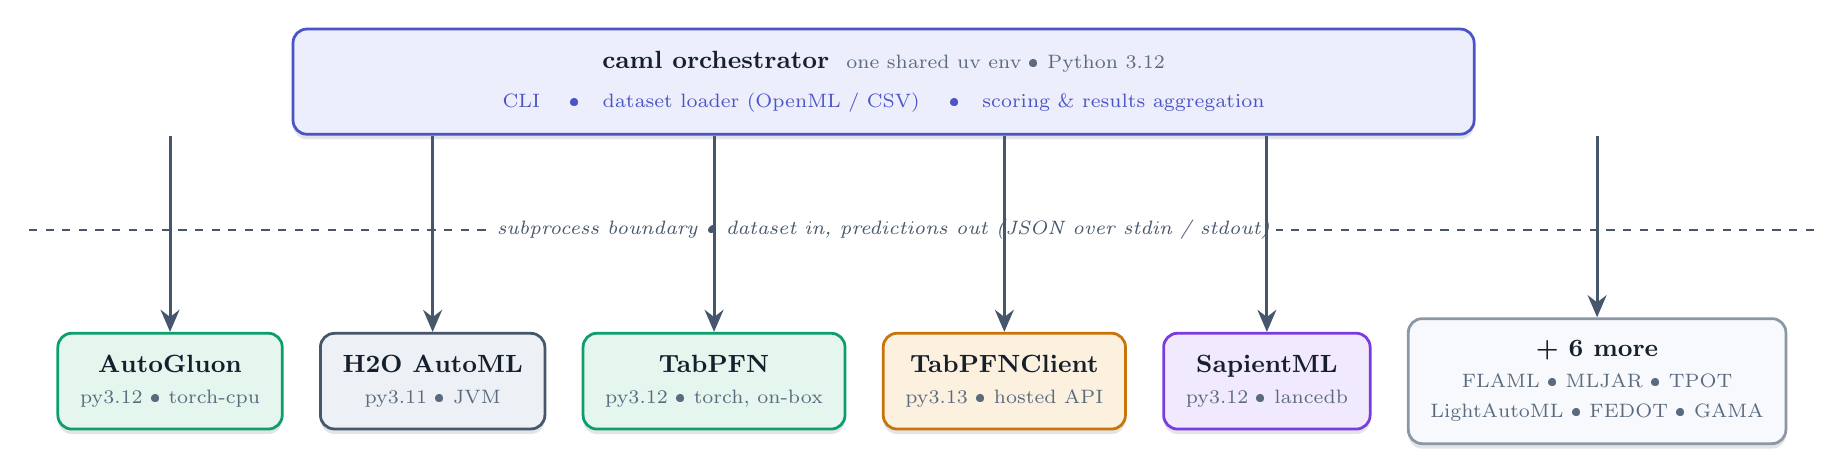
\begin{tikzpicture}

  % per-framework isolated venv cards
  \node[green]  (c1) {\Hd{AutoGluon}\\\Sb{py3.12 \textbullet\ torch-cpu}};
  \node[slate, right=0.45cm of c1]  (c2) {\Hd{H2O AutoML}\\\Sb{py3.11 \textbullet\ JVM}};
  \node[green, right=0.45cm of c2]  (c3) {\Hd{TabPFN}\\\Sb{py3.12 \textbullet\ torch, on-box}};
  \node[amber, right=0.45cm of c3]  (c4) {\Hd{TabPFNClient}\\\Sb{py3.13 \textbullet\ hosted API}};
  \node[purple, right=0.45cm of c4] (c5) {\Hd{SapientML}\\\Sb{py3.12 \textbullet\ lancedb}};
  \node[card, right=0.45cm of c5]   (c6) {\Hd{+ 6 more}\\\Sb{FLAML \textbullet\ MLJAR \textbullet\ TPOT}\\\Sb{LightAutoML \textbullet\ FEDOT \textbullet\ GAMA}};

  % orchestrator, centered above the row
  \coordinate (mid) at ($(c1.north)!0.5!(c6.north)$);
  \node[indigo, minimum width=15cm, above=2.4cm of mid, align=center] (orch)
    {\Hd{caml orchestrator}\ \ {\normalfont\scriptsize\textcolor{muted}{one shared uv env \textbullet\ Python 3.12}}\\[3pt]
     \Sbc{indigo}{CLI \quad\textbullet\quad dataset loader (OpenML / CSV) \quad\textbullet\quad scoring \& results aggregation}};

  % subprocess boundary the arrows cross
  \coordinate (bl) at ($(orch.south)!0.5!(mid)$);
  \draw[dashed, line width=0.9pt, edge]
    ($(c1.west |- bl)+(-0.35,0)$) -- ($(c6.east |- bl)+(0.35,0)$);
  \node[alabel, text=edge] at (bl)
    {\itshape subprocess boundary \textbullet\ dataset in, predictions out (JSON over stdin / stdout)};

  \foreach \c in {c1,c2,c3,c4,c5,c6}
    \draw[arrow] (orch.south -| \c) -- (\c.north);

\end{tikzpicture}
\end{document}
